\documentclass[10pt]{article}
% ---- NeurIPS-preprint-like layout (self-contained; no external style file) ----
\usepackage[letterpaper, textwidth=5.5in, textheight=9in, top=1in, headheight=12pt, headsep=25pt, footskip=30pt]{geometry}
\usepackage[T1]{fontenc}
\usepackage{newtxtext, newtxmath}
\usepackage{microtype, amsmath, booktabs, graphicx, xcolor, caption, subcaption, enumitem}
\usepackage[round, sort&compress]{natbib}
\usepackage{tikz}
\usetikzlibrary{arrows.meta, positioning, fit, calc}
\usepackage[colorlinks=true, linkcolor=blue!50!black, citecolor=blue!50!black, urlcolor=blue!50!black]{hyperref}
\usepackage{fancyhdr}
\pagestyle{fancy}\fancyhf{}\renewcommand{\headrulewidth}{0pt}
\fancyfoot[C]{\thepage}
\fancyfoot[L]{\footnotesize\textit{Preprint. Work in progress.}}
\captionsetup{font=small, labelfont=bf}
\setlist{itemsep=1pt, topsep=2pt}
\graphicspath{{figures/}}
% TikZ diagrams for the GENESIS paper (included from main.tex)

\newcommand{\systemdiagram}{%
\begin{tikzpicture}[font=\scriptsize, >=Stealth,
  box/.style={draw, rounded corners=2pt, align=center, minimum height=8mm, inner sep=3pt, fill=##1},
  box/.default=white, lab/.style={font=\tiny, align=center, text=black!70}]
  \node[box=green!8, minimum width=31mm] (world) {\textbf{World engine} (Numba)\\ 256$\times$256 island, seasons,\\ weather, fire/flood, fauna};
  \node[box=blue!6, right=12mm of world, minimum width=27mm] (obs) {\textbf{Egocentric perception}\\ 11$\times$11$\times$16 view (occluded)\\ + 13 body signals};
  \node[box=orange!10, right=12mm of obs, minimum width=28mm] (pol) {\textbf{Shared policy}\\ conv $\rightarrow$ GRU / MLP\\ one network, 256 bodies};
  \draw[->, thick] (world) -- node[lab, above]{state} (obs);
  \draw[->, thick] (obs) -- node[lab, above]{$o_t^i$} (pol);
  \draw[->, thick] (pol.south) -- ++(0,-6mm) -| node[lab, pos=0.25, below]{actions $a_t^i$ (move, eat, drink, rest, hunt, \dots)} (world.south);
  \node[box=red!6, above=7mm of obs, minimum width=56mm] (rew) {\textbf{Reward = own homeostasis only}: $r_t^i = D(h_t^i) - D(h_{t+1}^i) - \mathbf{1}[\text{death}]$};
  \draw[->, dashed] (world.north) |- (rew.west);
  \draw[->, dashed] (rew.east) -| (pol.north);
  \node[box=gray!8, below=14mm of obs, minimum width=56mm] (rec) {\textbf{Flight recorder}: every agent, every tick (position, body, action,\\ reward, death cause, value, action probabilities) $\rightarrow$ exact replay \& analysis};
  \draw[->, gray] (world.south) ++(-6mm,0) |- (rec.west);
\end{tikzpicture}}

\newcommand{\networkdiagram}{%
\begin{tikzpicture}[font=\scriptsize, >=Stealth, node distance=4mm,
  l/.style={draw, rounded corners=1.5pt, minimum height=6mm, align=center, inner sep=2pt, fill=##1}, l/.default=white]
  \node[l=blue!6] (g) {grid $11{\times}11{\times}16$};
  \node[l, right=of g] (c1) {conv 3$\times$3, 32};
  \node[l, right=of c1] (c2) {conv 3$\times$3/2, 64};
  \node[l, right=of c2] (fg) {fc 256};
  \node[l=blue!6, below=5mm of g] (v) {self 13 + nbrs 36 + heard 8};
  \node[l, right=of v, xshift=19mm] (fv) {fc 64};
  \node[l, right=12mm of fg, yshift=-5.5mm] (fc) {fc 256};
  \node[l=orange!12, right=of fc] (core) {GRU 256\\ \tiny (or MLP)};
  \node[l=green!10, right=of core, yshift=3.5mm] (pi) {$\pi(a\mid h)$, 11};
  \node[l=green!10, right=of core, yshift=-3.5mm] (vv) {$V(h)$};
  \draw[->] (g)--(c1); \draw[->] (c1)--(c2); \draw[->] (c2)--(fg); \draw[->] (v)--(fv);
  \draw[->] (fg.east)--(fc); \draw[->] (fv.east)--(fc); \draw[->] (fc)--(core);
  \draw[->] (core)--(pi); \draw[->] (core)--(vv);
  \draw[->, densely dotted] (core.south) -- ++(0,-4mm) -- ++(-7mm,0) node[below, font=\tiny]{$h_{t-1}$, reset at birth} -- ++(-0mm,0) |- (core.west);
\end{tikzpicture}}

\newcommand{\protocoldiagram}{%
\begin{tikzpicture}[font=\scriptsize, >=Stealth,
  s/.style={draw, rounded corners=2pt, minimum width=34mm, minimum height=7mm, align=center, fill=##1}]
  \node[s=green!8] (tr) {\textbf{Training worlds}\\ seeds $1000{+}100k{+}w$, new world / 40 it.};
  \node[s=yellow!12, right=6mm of tr] (va) {\textbf{Validation worlds}\\ seeds 500--502 (probes, curves)};
  \node[s=red!8, right=6mm of va] (te) {\textbf{Held-out test worlds}\\ seeds 0--4 (all reported claims)};
  \node[draw, dashed, rounded corners, fit=(tr)(va)(te), inner sep=3pt, label={[font=\tiny]above:same generator, disjoint seeds}] {};
  \node[below=5mm of va, font=\tiny, align=center] {hypotheses preregistered before evaluation $\cdot$ 5 seeds $\times$ 2 years $\times$ 256 agents $\cdot$
  bootstrap 95\% CIs + Hedges' $g$};
\end{tikzpicture}}

\newcommand{\ci}[3]{#1~\mbox{[#2,\,#3]}}

\title{\vspace{-0.4in}\rule{\textwidth}{3pt}\\[6pt]
\textbf{GENESIS: Survival-Only Learning Agents in a Seasonal Foraging Ecology}\\[2pt]
\large A testbed, baselines, and a behavioural anatomy of the first learners\\[-2pt]
\rule{\textwidth}{1pt}}
\author{%
  \textbf{Heet Ranpura}\thanks{Correspondence: \texttt{heetranpura1@gmail.com}.\quad Code: \url{https://github.com/HeetRanpura/Genesis}.}
  \qquad \textbf{Advik Divekar}}
\date{October 2026}

\begin{document}
\maketitle

\begin{abstract}
We ask what individual competence and social organisation emerge when minimally specified learning agents are
rewarded \emph{only} for keeping their own bodies alive. We introduce GENESIS, a fast, deterministic multi-agent
foraging ecology: a procedurally generated $256{\times}256$ island with rivers, seasons, weather, wildfire, floods,
famine, and food-limited prey and predator populations, in which every agent's reward is the reduction of its own
homeostatic drive (energy, hydration, health, warmth) and a death penalty. Social behaviour is never rewarded; it is
possible (food can be dropped and picked up; large prey need two hunters) but must emerge. We train a single
parameter-shared recurrent PPO policy for 256 bodies (19.7M agent-steps) and evaluate it, with hypotheses registered
in advance, on five held-out worlds against random, greedy and hand-written heuristic foragers. Learners cut
mortality by more than half relative to random and greedy agents (memoryless \ci{1.50}{1.30}{1.75},
GRU \ci{1.67}{1.45}{1.92} deaths per agent-year vs.\ random \ci{3.83}{3.53}{4.19}) and match, but do not beat, the
heuristic (\ci{1.50}{1.04}{2.11}); the result replicates across two independent implementations. A behavioural
analysis of every agent at every tick shows that learners discover \emph{graded homeostatic control} (the
probability of drinking rises from 0.09 when hydrated to 0.52 when parched), \emph{riverside sedentism} (median
2.0 cells from fresh water and 14-cell home ranges, vs.\ 3.6 and 38 for the heuristic), and a critic whose value
estimate tracks the body's distance from its set-point ($r=-0.65$ to $-0.75$). They never learn to hunt and die of
starvation in autumn and winter (76--77\% of deaths). Diet probes show this is a local optimum, not a property of the
world: plants alone cannot cover basal metabolism, while a hunting forager breaks even. Learners appear clustered,
but the clustering is fully explained by shared place preferences (nearest-neighbour ratio 0.84 against a habitat
null, 0.98--1.01 against a place-preference null): as preregistered, no social behaviour has emerged yet.
\end{abstract}

\section{Introduction}
Human sociality arose under survival pressure: finding water, surviving winter, hunting animals too large to take
alone. Whether comparable organisation arises in artificial agents that face similar pressures, \emph{without being
told to cooperate}, is a question about which parts of human social life are convergent outcomes of ecology and which
are contingent \citep{duenez2023social}. Agent-based models showed long ago that simple rules can generate trade,
migration and inequality \citep{epstein1996growing}, and deep multi-agent reinforcement learning has produced tool use
\citep{baker2020emergent}, bartering \citep{johanson2022bartering}, cooperation in social dilemmas
\citep{leibo2017multi, perolat2017common, leibo2021meltingpot} and emergent signalling
\citep{foerster2016learning, lazaridou2017multi}. Most of these results, however, either hand-code behaviour or shape
the reward (team rewards, explicit social or communication objectives), which makes it hard to say what the
\emph{ecology alone} produces.

GENESIS is built to answer that narrower question with unusually strict rules: (i) the reward is the agent's own
homeostasis \citep{keramati2014homeostatic} and nothing else; (ii) capabilities such as memory, communication,
reproduction and building are switches, off by default; (iii) every run is seeded and bit-reproducible; (iv)
non-learning baselines appear in every comparison; and (v) claims are made only on held-out worlds, with hypotheses
written down before evaluation. This paper reports the first learning agents in that setting and, because a single
mortality number hides \emph{how} agents survive, a detailed behavioural anatomy of what they learned.

\paragraph{Contributions.}
\begin{itemize}
  \item \textbf{GENESIS}, an open, deterministic, Numba-accelerated ecology (${\geq}100$k environment steps per
  minute with full observations for 1{,}000 agents on a laptop) with food-limited fauna, a flight recorder that
  logs every agent at every tick, and exact replay (\S\ref{sec:env}).
  \item \textbf{A preregistered evaluation} of parameter-shared recurrent PPO against three baselines on held-out
  worlds, replicated across two independent implementations (\S\ref{sec:results}).
  \item \textbf{A behavioural anatomy} of the learners: time budgets, need-conditioned choice, space use, daily and
  seasonal rhythms, critic internals, individual differences, and an aggregation test with a place-preference null
  (\S\ref{sec:behaviour}).
  \item \textbf{An energy-economy probe} showing the learners' plant-only diet is a local optimum the world does not
  force (\S\ref{sec:energy}).
\end{itemize}

\section{Related work}
\textbf{Artificial societies and artificial life.} Sugarscape \citep{epstein1996growing} grew social phenomena from
hand-written rules; Polyworld \citep{yaeger1994polyworld} evolved neural foragers. Neural MMO
\citep{suarez2019neural} provides a large survival world for many learning agents and is the closest modern platform;
GENESIS differs in its strictly homeostatic reward, ecological dynamics (seasons, food-limited fauna, disturbances),
held-out-world protocol and per-tick recording. Crafter \citep{hafner2022crafter} studies single-agent survival skills.
\textbf{Social learning in MARL.} Sequential social dilemmas \citep{leibo2017multi}, common-pool resources
\citep{perolat2017common} and Melting Pot \citep{leibo2021meltingpot} measure cooperation, usually with designed
incentives; cultural transmission \citep{bhoopchand2023learning} and bartering \citep{johanson2022bartering} emerge
in purpose-built tasks. LLM-agent societies \citep{park2023generative} start from human cultural priors, which our
agents lack by construction. \textbf{Homeostatic RL.} Defining reward as drive reduction toward physiological
set-points \citep{keramati2014homeostatic} grounds ``survival'' in a single, non-social objective.

\section{The GENESIS environment}\label{sec:env}
\begin{figure}[t]
  \centering
  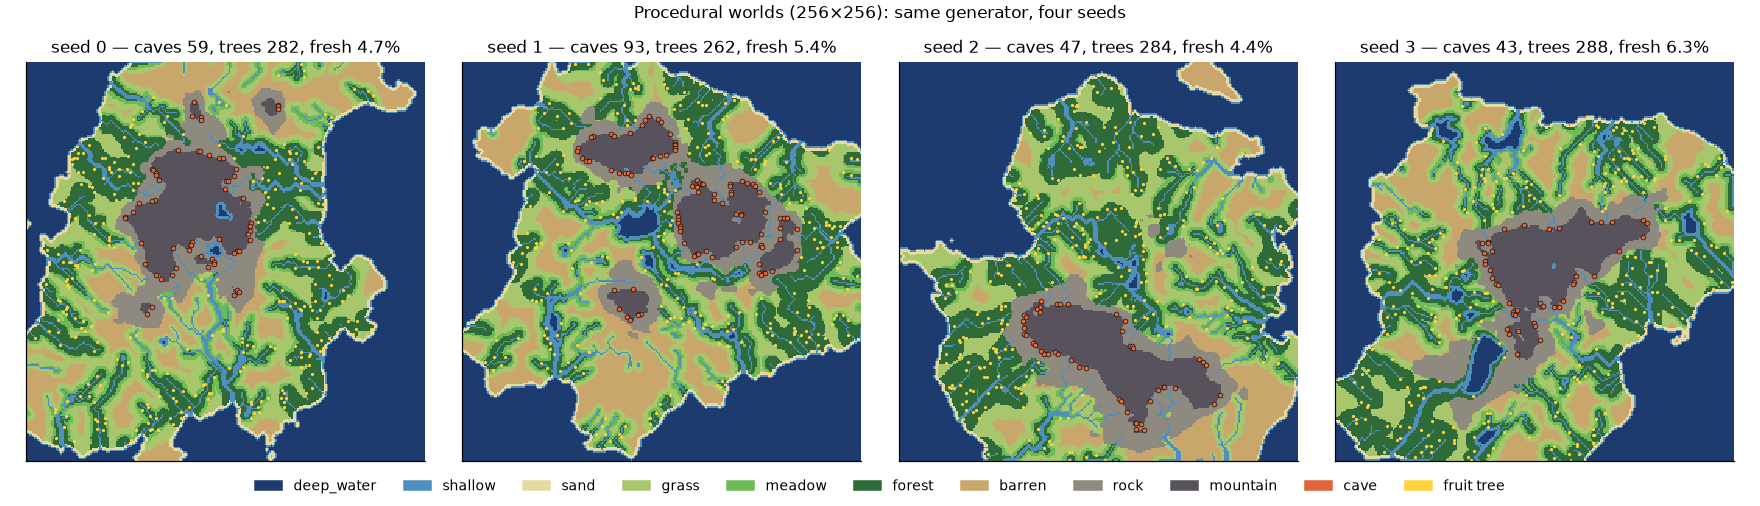
\includegraphics[width=\linewidth]{terrain.png}
  \caption{Four procedurally generated worlds (same generator, different seeds). Elevation from domain-warped fBm,
  lakes from priority-flood depression filling \citep{barnes2014priority}, rivers from flow accumulation; the ocean is
  salt, so fresh water is scarce and spatially structured. Red: caves; yellow: fruit trees.}
  \label{fig:terrain}
\end{figure}

\paragraph{World.} Each run generates a $256{\times}256$ island from its seed (Fig.~\ref{fig:terrain}) with ten
terrain classes. A year has four eight-day seasons of 120 ticks per day (3{,}840 ticks per year). Weather follows a
daily Markov chain (rain, fog, drought, cold snaps, snow); rare disturbances (wildfire, spring floods, famine years)
occur naturally and can be triggered. Plants regrow logistically toward a fertility map at seasonal rates; fruit trees
bear in one season; small prey, large prey and predators are \emph{food-limited}: they have energy stores, winter
torpor and seasonal breeding, and graze, flee, herd and hunt. Population caps exist only as safety rails and never
bind in our diagnostics. Each run starts after one year of ecological spin-up without agents.

\paragraph{Agents.} Agents occupy one cell each and perceive an $11{\times}11$ egocentric patch with 16 channels
(terrain, water, plants, fruit, prey, predators, other agents, fire, snow; line of sight blocked by mountains and dense
forest; the radius shrinks at night and in fog), 13 interoceptive signals, the four nearest visible neighbours, and
heard signals (unused here). Eleven actions: four moves, rest, eat, drink, hunt, pick up, drop, no-op. Bodies pay basal
metabolism (5.0 energy units per year), movement by terrain, and dehydration (faster in heat); health falls when
energy or water run out, when cold, in fire, or when attacked by predators. Large prey can be killed only by
${\geq}2$ attackers within six ticks, and carried food can be dropped where others can eat it. These features make
cooperation \emph{possible}; nothing rewards it.

\paragraph{Reward.} For agent $i$ with body $h^i\in[0,1]^4$ and set-point $h^*=(1,1,1,0.8)$, the drive is
$D(h)=\lVert\max(h^*-h,0)\rVert_2$ and the reward is $r^i_t = D(h^i_t)-D(h^i_{t+1})-\mathbf{1}[\text{death}]$
\citep{keramati2014homeostatic}. A unit test asserts that rewards depend only on the agent's own body.

\paragraph{Engineering.} The simulator is written in Numba \citep{lam2015numba}, is bit-reproducible across machines
(all randomness is a counter-based hash of seed, tick, index and stream), exposes a PettingZoo interface
\citep{terry2021pettingzoo}, and runs one tick as a single fused kernel call. Observations are masked copies of an
incrementally maintained observation image, which keeps 1{,}000 fully observing agents above 100k steps per minute on
a fanless laptop. A flight recorder stores every agent's state, action, reward and death cause at every tick (and,
for learners, the value estimate and action probabilities), and any run can be replayed bit-exactly.

\begin{figure}[t]
  \centering
  \resizebox{\linewidth}{!}{\systemdiagram}
  \caption{The GENESIS loop. One shared policy drives every body; each agent's reward depends only on its own
  homeostasis; every tick of every agent is recorded.}
  \label{fig:system}
\end{figure}

\section{Agents and protocol}\label{sec:protocol}
\paragraph{Baselines.} \emph{Random} samples actions uniformly. \emph{Greedy} attends to its lower of energy and
hydration and walks to the nearest visible resource for it, else explores. \emph{Heuristic} is a hand-written
survivalist: it flees predators and fire, drinks and eats with hysteresis thresholds, hunts adjacent small prey, seeks
shelter when cold, and rests at night. None has a social rule.

\paragraph{Learner.} One actor-critic network (Fig.~\ref{fig:network}; about 1.1M parameters) is shared by all 256
agents; each agent keeps its own recurrent state, reset when a newborn takes over its slot. The core is a GRU
\citep{cho2014learning} (\emph{memory}) or a feed-forward layer (\emph{memoryless} ablation). We train with PPO
\citep{schulman2017proximal} and GAE \citep{schulman2016gae} on 128-tick rollouts of 256 agents, back-propagating
through whole rollouts, for 600 iterations (19.7M agent-steps; Appendix Table~\ref{tab:hparams}). A death cuts the
bootstrap. Action sampling is seeded on the CPU, so training is deterministic on CPU; the GPU (Apple MPS) path is not
bit-exact.

\begin{figure}[t]
  \centering
  \resizebox{0.95\linewidth}{!}{\networkdiagram}
  \caption{The shared actor-critic. The core is a GRU (memory) or an MLP (memoryless ablation).}
  \label{fig:network}
\end{figure}

\paragraph{Protocol.} Training worlds use seeds $1000+100k+w$ (a new world every 40 iterations), validation worlds
seeds 500--502 (probes and curves), and held-out test worlds seeds 0--4, never seen in training
(Fig.~\ref{fig:protocol}). Every evaluation uses 256 agents for two years on each of the five test worlds with a fixed
population (dead agents are replaced by newcomers with random genes). We report deaths per agent-year and
Kaplan--Meier survival \citep{kaplan1958nonparametric} with 95\% bootstrap confidence intervals over worlds
\citep{efron1993bootstrap} and Hedges' $g$ \citep{hedges1981distribution}. Four hypotheses were registered before
the first evaluation: \textbf{H1} learners beat random and greedy; \textbf{H2} learners beat the heuristic;
\textbf{H3} memory reduces thirst deaths without increasing overall mortality; \textbf{H4} no social behaviour beyond
what shared resources explain. ``Beats'' requires non-overlapping CIs.

\begin{figure}[h]
  \centering
  \resizebox{\linewidth}{!}{\protocoldiagram}
  \caption{World splits. All reported claims use the held-out test worlds.}
  \label{fig:protocol}
\end{figure}

\section{Results: survival}\label{sec:results}
\begin{table}[t]
  \centering\small
  \caption{Held-out worlds (seeds 0--4, 2 years, 256 agents). Mean with 95\% bootstrap CI over worlds; $g$: Hedges'
  $g$ of learner minus heuristic on per-world mortality (positive = more deaths).}
  \label{tab:main}
  \begin{tabular}{lccccc}
    \toprule
    Policy & deaths / agent-year & KM survival at 1 yr & starvation & thirst & $g$ vs heuristic \\
    \midrule
    Random & \ci{3.83}{3.53}{4.19} & 0.001 & 52\% & 34\% & --- \\
    Greedy & \ci{3.31}{2.92}{3.77} & 0.006 & 18\% & 61\% & --- \\
    Heuristic & \ci{1.50}{1.04}{2.11} & 0.214 & 9\% & 62\% & --- \\
    \midrule
    PPO memoryless & \ci{1.50}{1.30}{1.75} & 0.100 & 76\% & 10\% & $+0.01$ \\
    PPO GRU & \ci{1.67}{1.45}{1.92} & 0.055 & 77\% & 6\% & $+0.31$ \\
    \midrule
    \multicolumn{6}{l}{\emph{Original independent implementation (same protocol, different code)}} \\
    PPO memoryless & \ci{1.58}{1.35}{1.83} & 0.101 & 71\% & 15\% & $+0.15$ \\
    PPO GRU & \ci{1.80}{1.52}{2.10} & 0.062 & 79\% & 5\% & $+0.50$ \\
    \bottomrule
  \end{tabular}
\end{table}

\begin{figure}[t]
  \centering
  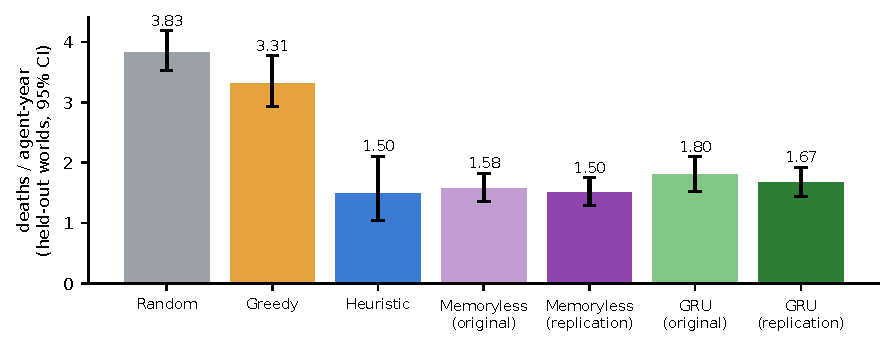
\includegraphics[width=\linewidth]{heldout_mortality.pdf}\\[2pt]
  \begin{subfigure}{0.49\linewidth}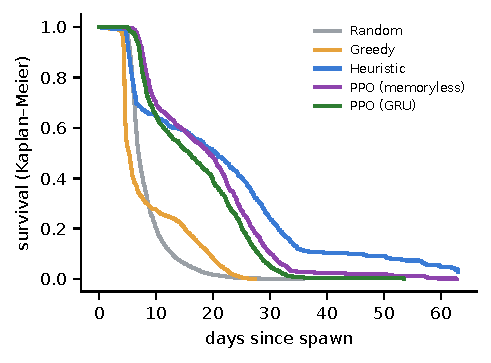
\includegraphics[width=\linewidth]{survival_km.pdf}\caption{Survival (test world 0)}\end{subfigure}
  \begin{subfigure}{0.49\linewidth}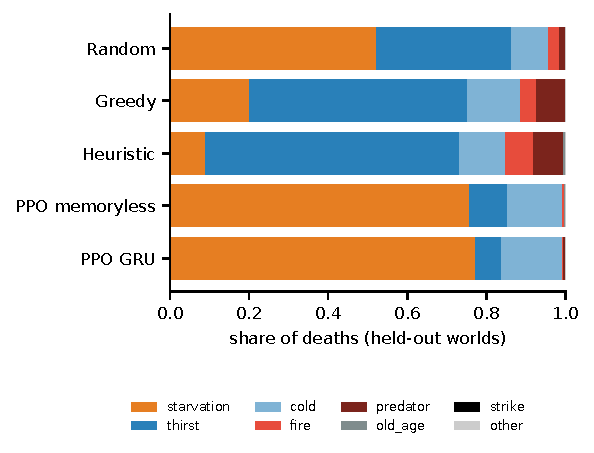
\includegraphics[width=\linewidth]{causes.pdf}\caption{Causes of death (all test worlds)}\end{subfigure}
  \caption{\textbf{Top:} held-out mortality, including the original implementation and our replication.
  \textbf{Bottom:} learners trade thirst and predator deaths for starvation.}
  \label{fig:mortality}
\end{figure}

\paragraph{H1 supported, H2 not supported.} Both learners more than halve mortality relative to random and greedy
agents (Table~\ref{tab:main}, Fig.~\ref{fig:mortality}; $g$ from $-3.4$ to $-5.7$) with non-overlapping CIs. Neither
is distinguishable from the heuristic at five worlds. Kaplan--Meier survival at one year is lower for learners than
for the heuristic despite similar death rates, because learners' deaths are concentrated in autumn and winter
(\S\ref{sec:behaviour}).

\paragraph{The causes of death change completely.} Learners almost eliminate thirst (6--10\% of deaths vs.\ 62\% for
the heuristic), fire and predator deaths, and instead die of starvation (76--77\%). They have solved the problems
that kill the hand-written agent and are now limited by energy.

\paragraph{Replication across implementations.} The results were first obtained with an independent implementation
of the same learner and protocol; after merging the two code bases into one trainer, we retrained both arms from
scratch. All four estimates overlap (Table~\ref{tab:main}), the ordering (memoryless $\leq$ GRU) and the
cause-of-death profile repeat, and the replication's point estimates are slightly better.

\paragraph{H3: memory does not help yet.} With memory, thirst deaths fall (6\% vs.\ 10\%; in the original run 5\%
vs.\ 15\%), but overall mortality is not lower; the memoryless agent is better on point estimates in both
implementations. At 19.7M agent-steps the GRU's advantage for remembering out-of-view water is outweighed by its
higher cost of learning; H3 is \emph{not supported} at this budget.

\paragraph{Training dynamics.} Policy entropy falls steadily from 2.40 (uniform) to 1.33--1.39 nats
(Fig.~\ref{fig:training}). Training-world mortality is dominated by the world schedule and seasons and is not a
usable learning curve; we have since added periodic evaluation on fixed validation worlds.

\begin{figure}[t]
  \centering
  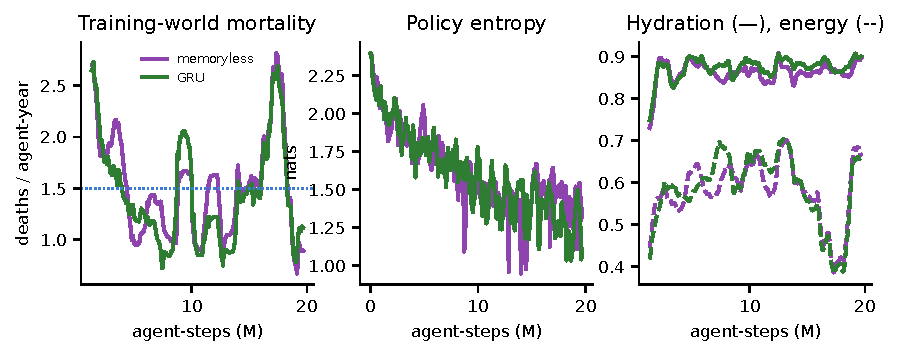
\includegraphics[width=\linewidth]{training.pdf}
  \caption{Training. Mortality on training worlds (40-iteration mean; dotted: heuristic's held-out rate) oscillates
  with world switches and seasons; entropy falls steadily; hydration rises early, energy stays seasonal.}
  \label{fig:training}
\end{figure}

\section{A behavioural anatomy of the learners}\label{sec:behaviour}
All analyses in this section use the complete per-tick recordings of test world 0 (two years, 256 agents
continuously, ${\approx}2$M agent-ticks per policy) and compare all five policies on the same world.

\paragraph{Time budget: forage little and often.} The heuristic moves 58\% of the time and rests 38\%, eating in 4\%
and drinking in 0.5\% of ticks (large meals triggered by thresholds). Learners move \emph{less} (27--35\%), rest 21--28\%,
and spend 20--23\% of ticks eating and 10--11\% drinking (Fig.~\ref{fig:budget}a): many small meals and sips.

\paragraph{Graded homeostatic control.} The probability of drinking is a smooth, monotone function of the agent's own
hydration: from 0.52 when parched to 0.09 when sated for the memoryless learner (0.35 to 0.09 with memory;
Fig.~\ref{fig:budget}b). Eating is U-shaped: learners eat most when hungry but also when almost full (0.25 at the top
energy decile), where part of the intake is wasted against the energy cap. This explains a paradox in
\S\ref{sec:energy}: learners \emph{eat more} than any hand-written forager yet starve.

\begin{figure}[t]
  \centering
  \begin{subfigure}{0.36\linewidth}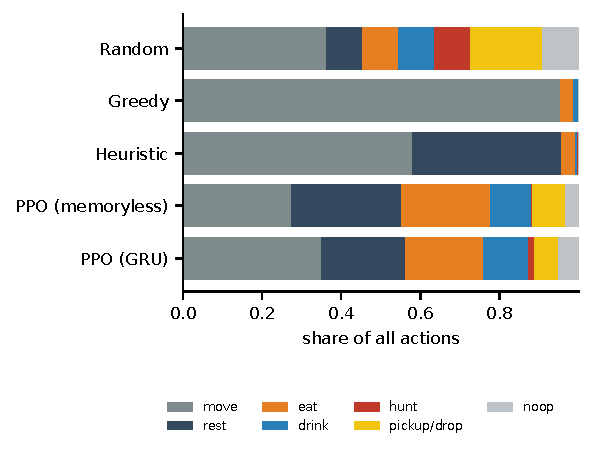
\includegraphics[width=\linewidth]{action_budget.pdf}\caption{Action budget}\end{subfigure}\hfill
  \begin{subfigure}{0.62\linewidth}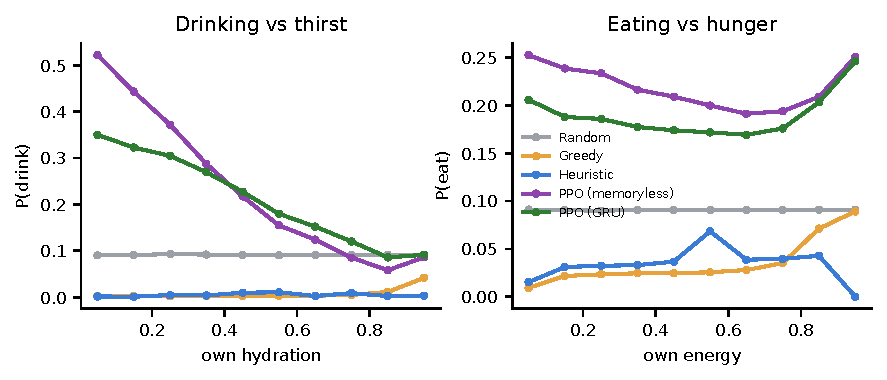
\includegraphics[width=\linewidth]{homeostatic_control.pdf}\caption{Need-conditioned choice}\end{subfigure}
  \caption{\textbf{(a)} Learners forage in many small bites. \textbf{(b)} Drinking rises smoothly with thirst;
  eating is U-shaped in energy. Baselines are flat (random) or near zero per tick (threshold-driven heuristic).}
  \label{fig:budget}
\end{figure}

\paragraph{Riverside sedentism.} Learners stay close to fresh water: median 2.0--2.2 cells, vs.\ 3.6 for the heuristic and
4.2 for random and greedy agents. They keep small home ranges (median radius of gyration 14--18 cells vs.\ 35--38 for
heuristic and greedy agents; Fig.~\ref{fig:space}). Occupancy maps show them threading along the river network: a
\emph{central-place} strategy that guarantees water and lets plants near rivers regrow between visits.

\begin{figure}[t]
  \centering
  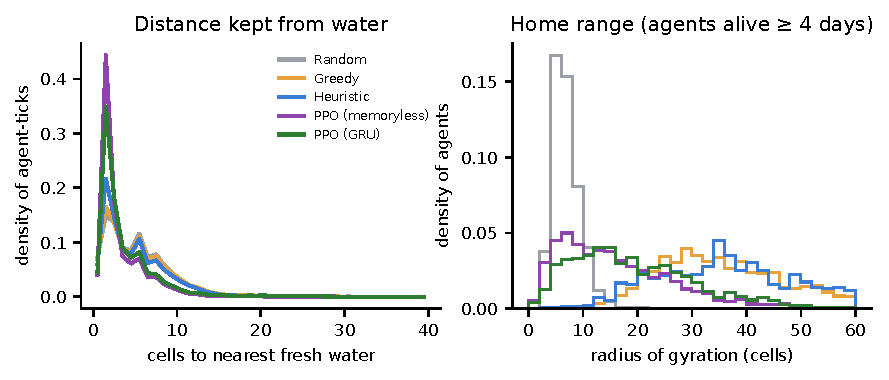
\includegraphics[width=\linewidth]{water_homerange.pdf}\\
  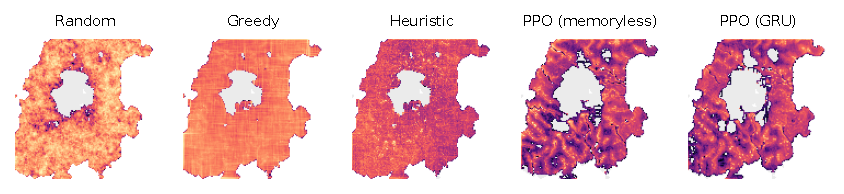
\includegraphics[width=\linewidth]{occupancy.pdf}
  \caption{Space use on test world 0. \textbf{Top:} distance kept from fresh water and home-range size.
  \textbf{Bottom:} where each policy spent its time (log visits). Learners concentrate along rivers.}
  \label{fig:space}
\end{figure}

\paragraph{Daily and seasonal rhythms.} The heuristic rests at night by construction (69\% at night vs.\ 8\% at midday).
Learners show \emph{no} night-time resting (memoryless 25\% at night vs.\ 31\% at midday;
Fig.~\ref{fig:rhythms}a), so the world's darkness (shorter sight, colder air) has not been exploited. Seasonally,
learners' mean energy peaks in summer (0.75--0.79) and collapses through autumn (0.42--0.46) into winter
(0.30--0.33), when plant growth stops; the heuristic, which hunts, keeps 0.69 in autumn and 0.50 in winter. Learner
deaths are concentrated in autumn and winter (Fig.~\ref{fig:rhythms}b).

\begin{figure}[t]
  \centering
  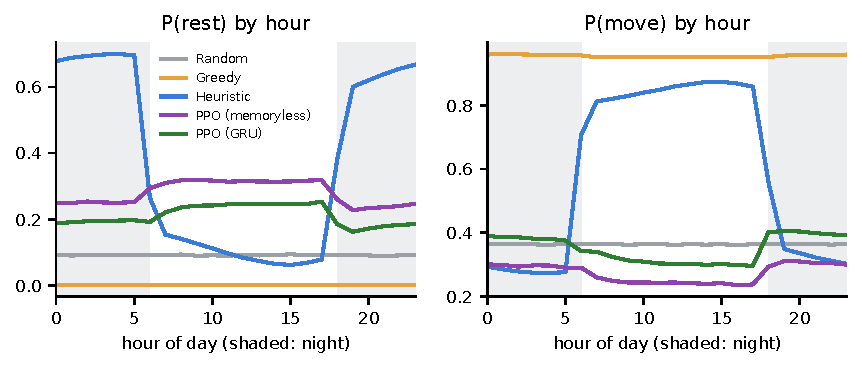
\includegraphics[width=\linewidth]{circadian.pdf}\\
  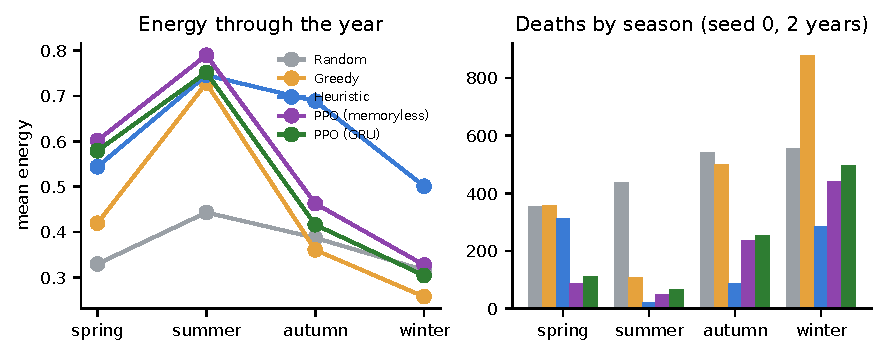
\includegraphics[width=\linewidth]{seasonal.pdf}
  \caption{\textbf{Top:} resting and moving by hour (shaded: night). Only the hand-written heuristic rests at night.
  \textbf{Bottom:} energy through the year and deaths by season. Learners starve when plant growth stops.}
  \label{fig:rhythms}
\end{figure}

\paragraph{What the critic tracks.} The learned value estimate falls monotonically with the body's distance from its
set-point ($r=-0.65$ memoryless, $-0.75$ GRU; Fig.~\ref{fig:internals}) and is lower in autumn and winter: the critic
has learned an interoceptive ``well-being'' signal from the reward alone. The GRU's policy becomes markedly more
decisive at dawn (entropy 1.43 at night $\rightarrow$ 1.23 at 06:00), a temporal structure absent from the memoryless
policy (1.44--1.50 throughout).

\begin{figure}[t]
  \centering
  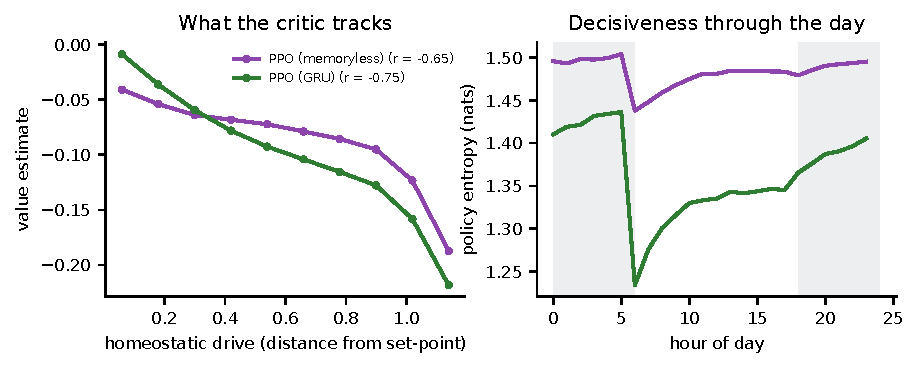
\includegraphics[width=\linewidth]{internals.pdf}
  \caption{Learner internals. \textbf{Left:} value estimate against homeostatic drive. \textbf{Right:} policy entropy by
  hour; the GRU policy sharpens at dawn.}
  \label{fig:internals}
\end{figure}

\paragraph{Individual differences.} Although every agent runs the same network, individuals differ in state and
history. We embed each agent that lived at least four days by its action frequencies
(Fig.~\ref{fig:social}a). Policies separate cleanly; \emph{within} a policy, k-means finds only weakly separated groups
(best silhouette 0.34 memoryless, 0.41 GRU, 0.43 heuristic, against 0.11 for random agents). There is a continuum of
movers and grazers, but no evidence of distinct behavioural roles.

\paragraph{Social structure: H4 holds.} Learners are closer to each other than to random points drawn from the cells they
use (nearest-neighbour ratio 0.84 vs.\ 0.95--0.98 for baselines; Fig.~\ref{fig:social}b), which could be read as
aggregation. A stronger null that preserves each policy's own place preferences (points drawn in proportion to visits)
removes the effect entirely (0.98--1.01). Learners cluster because they favour the same riverbanks, not because they
are attracted to one another. Across all five test worlds (${\approx}2{,}560$ agent-years per policy) learners
made \emph{no} successful group kill of large prey (5 and 12 attack attempts), and food left by another agent
supplied 11.4 (memoryless) and 24.5 (GRU) energy units in total, under 0.01 per agent-year against an intake of
${\approx}6.5$. That is less than the incidental scavenging of the rule-based heuristic, which has no social rule
(65.6). We find no social behaviour at this stage, as preregistered.

\begin{figure}[t]
  \centering
  \begin{subfigure}{0.5\linewidth}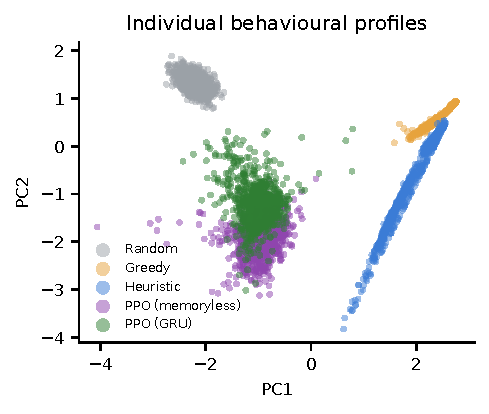
\includegraphics[width=\linewidth]{individuals.pdf}\caption{Behavioural profiles (PCA)}\end{subfigure}\hfill
  \begin{subfigure}{0.48\linewidth}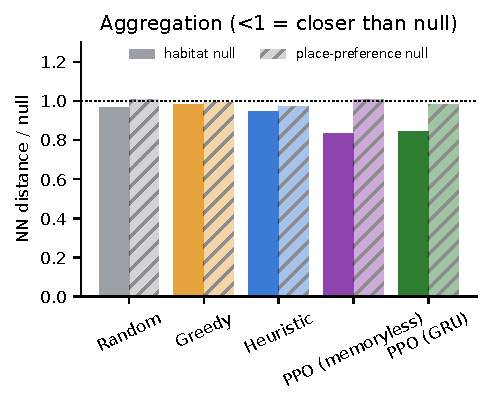
\includegraphics[width=\linewidth]{aggregation.pdf}\caption{Aggregation vs.\ two nulls}\end{subfigure}
  \caption{\textbf{(a)} Each dot is one agent's lifetime action profile; policies separate, individuals within a
  learner policy form a continuum. \textbf{(b)} Apparent learner aggregation against a habitat null disappears under a
  place-preference null.}
  \label{fig:social}
\end{figure}

\section{Is starvation forced by the world? An energy-economy probe}\label{sec:energy}
Learners eat plants and fruit and almost never hunt. To ask whether that is a limitation of the world or of learning,
we ran hand-written foragers that differ \emph{only} in what a hungry agent seeks (identical water, shelter and
danger rules) on the validation worlds (three seeds, two years), together with the learners (Fig.~\ref{fig:energy}).

\begin{figure}[t]
  \centering
  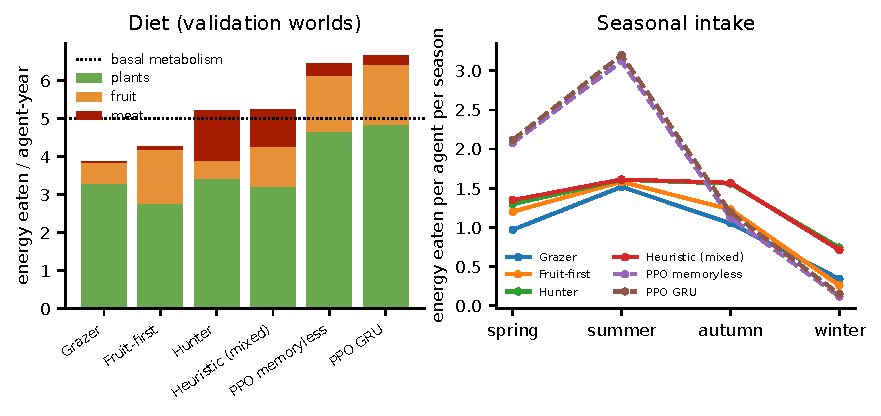
\includegraphics[width=\linewidth]{energy.pdf}
  \caption{Energy economy on validation worlds. \textbf{Left:} energy eaten per agent-year by source; dotted line:
  basal metabolism alone. \textbf{Right:} seasonal intake. Plant-only grazing cannot sustain a body; adding meat closes
  the winter gap.}
  \label{fig:energy}
\end{figure}

A pure grazer eats 3.9 energy units per agent-year, \emph{below} basal metabolism (5.0), and dies at 3.12 per
agent-year. A fruit-first forager does little better (4.3; 2.58). Adding hunting closes the gap: the hunter eats
5.2 (1.3 of it meat) and dies at 1.33, and the mixed heuristic eats 5.3 and dies at 1.24. Meat matters most in winter,
when plant intake collapses (Fig.~\ref{fig:energy}, right). Over the year the learners eat more than any
hand-written forager (6.4--6.7, mostly plants and fruit), but the timing is wrong. They eat twice the heuristic's
intake in spring and summer (2.1 and 3.1--3.2 units per agent per season, vs.\ 1.35 and 1.6), much of it near the
energy cap where it is wasted. In winter they eat 0.12--0.15, less than a fifth of the heuristic's 0.71, because meat is
the only food that does not stop growing in winter and they take almost none (0.24--0.30 per agent-year). Their
deaths are 75--77\% starvation, concentrated in autumn and winter. \textbf{The world rewards hunting; the learners have not found it.} Their
diet is a local optimum, consistent with the credit-assignment difficulty of hunting (approach, repeated attacks,
eating the carcass, with no reward until the energy arrives).

\section{Discussion}
\paragraph{What emerged.} From a purely homeostatic reward, a single shared network learned interoceptive control
(graded drinking and eating), a central-place foraging strategy anchored on rivers, and a critic that represents
bodily well-being and season. Structurally, this resembles the water-tethered foraging of many mobile animals and of
human foragers in arid environments. We offer this only as an analogy: it is the expected solution to a water-limited
landscape, not evidence of human-like cognition.

\paragraph{What did not emerge.} Hunting, night-time rest, food sharing, cooperative hunting and aggregation beyond
shared place preference are all absent. The world makes each of them possible: group kills of large prey require
two hunters, and dropped food can be taken. Their absence at 20M agent-steps sets a clear bar for what later
capabilities (longer training, memory, communication, reproduction) must change. The energy probe shows the next
bottleneck is ecological competence (hunting), which plausibly precedes any social use of meat. This ordering,
\emph{individual hunting before sharing}, is itself a testable prediction.

\paragraph{Limitations.}
\begin{itemize}
  \item \textbf{Seeds and budget:} one training seed per arm and 19.7M agent-steps, small for a 1.1M-parameter
  recurrent policy. H2 and H3 may change with more training.
  \item \textbf{Scope of the behavioural analysis:} it uses one test world. The aggregate statistics use all five.
  \item \textbf{Reproducibility:} MPS (GPU) arithmetic is not bit-exact, so the learner replication is statistical.
  The simulator itself is bit-exact.
  \item \textbf{Design choices:} the world's parameters (metabolism, prey energy, fauna dynamics) shape every result.
  We report the energy probe rather than retune the world for the learners.
  \item \textbf{Population model:} the fixed-population, respawn protocol has no reproduction or inheritance, so
  nothing here speaks to cultural or genetic accumulation.
\end{itemize}

\paragraph{Next steps.} Longer runs ($\geq$100M agent-steps, three seeds per arm) with periodic validation; curricula
or intrinsic-motivation ablations to test whether hunting is an exploration problem; then the Stage 3 social metrics
(co-feeding, food transfer, signal--context information) under the reproduction and communication switches.

\paragraph{Reproducibility and broader impact.} Code, configurations, preregistration, evaluation files and analysis
scripts are public. Every number in this paper is produced by scripts in the repository (\texttt{eval\_policy.py},
\texttt{energy\_economy.py}, \texttt{behaviour\_analysis.py}, \texttt{paper\_figures.py}). The work studies artificial
agents in a simulated ecology and carries no direct societal risk. We caution against reading structural analogies with
human prehistory as claims about humans.

\begin{thebibliography}{30}\small
\bibitem[Baker et~al.(2020)]{baker2020emergent} B.~Baker, I.~Kanitscheider, T.~Markov, Y.~Wu, G.~Powell, B.~McGrew, and I.~Mordatch. Emergent tool use from multi-agent autocurricula. In \emph{ICLR}, 2020.
\bibitem[Barnes et~al.(2014)]{barnes2014priority} R.~Barnes, C.~Lehman, and D.~Mulla. Priority-flood: an optimal depression-filling and watershed-labeling algorithm for digital elevation models. \emph{Computers \& Geosciences}, 62:117--127, 2014.
\bibitem[Bhoopchand et~al.(2023)]{bhoopchand2023learning} A.~Bhoopchand et~al. Learning few-shot imitation as cultural transmission. \emph{Nature Communications}, 14, 2023.
\bibitem[Cho et~al.(2014)]{cho2014learning} K.~Cho, B.~van Merri\"enboer, C.~Gulcehre, D.~Bahdanau, F.~Bougares, H.~Schwenk, and Y.~Bengio. Learning phrase representations using RNN encoder-decoder for statistical machine translation. In \emph{EMNLP}, 2014.
\bibitem[Du\'e\~nez-Guzm\'an et~al.(2023)]{duenez2023social} E.~A. Du\'e\~nez-Guzm\'an, S.~Sadedin, J.~X. Wang, K.~R. McKee, and J.~Z. Leibo. A social path to human-like artificial intelligence. \emph{Nature Machine Intelligence}, 5:1181--1188, 2023.
\bibitem[Efron and Tibshirani(1993)]{efron1993bootstrap} B.~Efron and R.~J. Tibshirani. \emph{An Introduction to the Bootstrap}. Chapman \& Hall, 1993.
\bibitem[Epstein and Axtell(1996)]{epstein1996growing} J.~M. Epstein and R.~Axtell. \emph{Growing Artificial Societies: Social Science from the Bottom Up}. MIT Press, 1996.
\bibitem[Foerster et~al.(2016)]{foerster2016learning} J.~N. Foerster, Y.~M. Assael, N.~de~Freitas, and S.~Whiteson. Learning to communicate with deep multi-agent reinforcement learning. In \emph{NeurIPS}, 2016.
\bibitem[Hafner(2022)]{hafner2022crafter} D.~Hafner. Benchmarking the spectrum of agent capabilities. In \emph{ICLR}, 2022.
\bibitem[Hedges(1981)]{hedges1981distribution} L.~V. Hedges. Distribution theory for Glass's estimator of effect size and related estimators. \emph{Journal of Educational Statistics}, 6(2):107--128, 1981.
\bibitem[Johanson et~al.(2022)]{johanson2022bartering} M.~B. Johanson, E.~Hughes, F.~Timbers, and J.~Z. Leibo. Emergent bartering behaviour in multi-agent reinforcement learning. \emph{arXiv:2205.06760}, 2022.
\bibitem[Kaplan and Meier(1958)]{kaplan1958nonparametric} E.~L. Kaplan and P.~Meier. Nonparametric estimation from incomplete observations. \emph{Journal of the American Statistical Association}, 53(282):457--481, 1958.
\bibitem[Keramati and Gutkin(2014)]{keramati2014homeostatic} M.~Keramati and B.~Gutkin. Homeostatic reinforcement learning for integrating reward collection and physiological stability. \emph{eLife}, 3:e04811, 2014.
\bibitem[Lam et~al.(2015)]{lam2015numba} S.~K. Lam, A.~Pitrou, and S.~Seibert. Numba: a LLVM-based Python JIT compiler. In \emph{LLVM-HPC Workshop}, 2015.
\bibitem[Lazaridou et~al.(2017)]{lazaridou2017multi} A.~Lazaridou, A.~Peysakhovich, and M.~Baroni. Multi-agent cooperation and the emergence of (natural) language. In \emph{ICLR}, 2017.
\bibitem[Leibo et~al.(2017)]{leibo2017multi} J.~Z. Leibo, V.~Zambaldi, M.~Lanctot, J.~Marecki, and T.~Graepel. Multi-agent reinforcement learning in sequential social dilemmas. In \emph{AAMAS}, 2017.
\bibitem[Leibo et~al.(2021)]{leibo2021meltingpot} J.~Z. Leibo et~al. Scalable evaluation of multi-agent reinforcement learning with Melting Pot. In \emph{ICML}, 2021.
\bibitem[Park et~al.(2023)]{park2023generative} J.~S. Park, J.~C. O'Brien, C.~J. Cai, M.~R. Morris, P.~Liang, and M.~S. Bernstein. Generative agents: interactive simulacra of human behavior. In \emph{UIST}, 2023.
\bibitem[Perolat et~al.(2017)]{perolat2017common} J.~Perolat, J.~Z. Leibo, V.~Zambaldi, C.~Beattie, K.~Tuyls, and T.~Graepel. A multi-agent reinforcement learning model of common-pool resource appropriation. In \emph{NeurIPS}, 2017.
\bibitem[Schulman et~al.(2016)]{schulman2016gae} J.~Schulman, P.~Moritz, S.~Levine, M.~Jordan, and P.~Abbeel. High-dimensional continuous control using generalized advantage estimation. In \emph{ICLR}, 2016.
\bibitem[Schulman et~al.(2017)]{schulman2017proximal} J.~Schulman, F.~Wolski, P.~Dhariwal, A.~Radford, and O.~Klimov. Proximal policy optimization algorithms. \emph{arXiv:1707.06347}, 2017.
\bibitem[Suarez et~al.(2019)]{suarez2019neural} J.~Suarez, Y.~Du, P.~Isola, and I.~Mordatch. Neural MMO: a massively multiagent game environment for training and evaluating intelligent agents. \emph{arXiv:1903.00784}, 2019.
\bibitem[Terry et~al.(2021)]{terry2021pettingzoo} J.~K. Terry et~al. PettingZoo: Gym for multi-agent reinforcement learning. In \emph{NeurIPS}, 2021.
\bibitem[Yaeger(1994)]{yaeger1994polyworld} L.~Yaeger. Computational genetics, physiology, metabolism, neural systems, learning, vision, and behavior or PolyWorld: life in a new context. In \emph{Artificial Life III}, 1994.
\end{thebibliography}

\appendix
\section{Hyperparameters and environment settings}
\begin{table}[h]
  \centering\small
  \caption{Learner hyperparameters (identical for both arms except the core).}
  \label{tab:hparams}
  \resizebox{\linewidth}{!}{%
  \begin{tabular}{ll@{\qquad}ll}
    \toprule
    Agents (shared policy) & 256 & Rollout length & 128 ticks \\
    Iterations & 600 (19.7M agent-steps) & BPTT & whole rollout \\
    Discount $\gamma$ / GAE $\lambda$ & 0.995 / 0.95 & Epochs $\times$ minibatches & $4\times4$ (split by agent) \\
    Clip / entropy / value coef. & 0.2 / 0.01 / 0.5 & Optimiser & Adam, lr $3\cdot10^{-4}$, grad.\ clip 0.5 \\
    Hidden size & 256 (GRU or MLP core) & Reward & raw homeostatic (no normalisation) \\
    Training worlds & $1000{+}w$, new world / 40 it. & Hardware & Apple M-series laptop, MPS \\
    Wall time & 1.0 h (memoryless), 1.7 h (GRU) & Parameters & ${\approx}1.1$M \\
    \bottomrule
  \end{tabular}}
\end{table}

\paragraph{Environment.} Basal metabolism 0.0013 energy per tick; plant bite 0.25 biomass $\rightarrow$ 0.03 energy;
fruit 0.15; small-prey carcass 0.30 (60\% kill chance per hunt action); large-prey carcass 1.8 (two attackers within six
ticks); predators attack adjacent agents with probability 0.4 for 0.08 health. Fauna: energy stores, metabolism
$\times0.2$ below 5\,\textdegree C, births in spring to autumn only; caps and immigration floors never bind in diagnostics
(5 seeds $\times$ 3 years). Full specification: \texttt{docs/WORLD.md}; all values: \texttt{configs/default.yaml}.

\paragraph{Diet probes.} The four hand-written foragers share every rule of the heuristic (flee predators and fire,
drink with hysteresis, seek shelter when cold, rest at night) and differ only in what a hungry agent seeks: plants only
(grazer), fruit trees first (fruit-first), small prey first (hunter), or the heuristic's default order (mixed). The
heuristic's standard path reproduces its committed baseline bit-for-bit.
\end{document}
